\textbf{\underline{OZ 6 - Magnetische inductie en de wet van Faraday - Oefening 1:}}
\vspace{0.5cm}

    \begin{minipage}{.8\textwidth}
        Een kort stuk van een draad, van lengte $a$, beweegt met snelheid $\vec{v}$ , parallel langs
        een zeer lange draad waardoor een stroom $I$ loopt d. Het dichtste uiteinde
        van de korte draad is een afstand b van de lange draad verwijderd. Neem aan dat de
        verticale draad lang is vergeleken met a + b. Bepaal de emf tussen de uiteindes van
        de korte draad wanneer $\vec{v}$ 

        \begin{enumerate}[(a)]
            \item in de zelfde zin is als I,
            \item in de tegengestelde zin is als $I$.
        \end{enumerate}

    \end{minipage}
    \hspace{0.5cm}\begin{minipage}{.16\textwidth}
        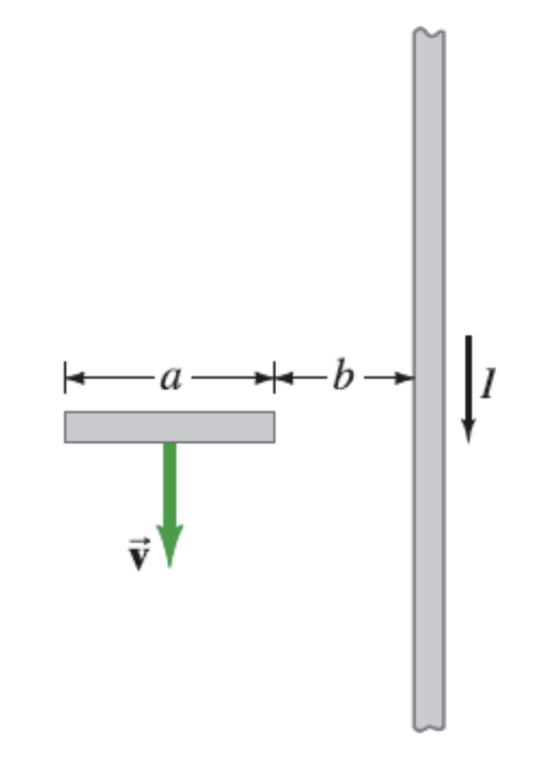
\includegraphics[scale = 0.28]{oz06/resources/Oz6Oef1.png}
    \end{minipage}

    \begin{enumerate}[(a)]
        \item     
            \begin{description}[labelwidth=1.5cm, leftmargin=!]
                \item[Geg. :] $v$, $I$, $a$, $b$
                \item[Gevr. :] $\mathcal{E}_{\text{ind}}$
                \item[Opl. :]
                \item[] 
                    \vspace{-0.45cm}\begin{minipage}{.6\textwidth}
                        Het magnetische veld van de lange draad gaat in het blad, maar het verkleint hoe verder we van de draad weggaan.
                        We berekenen de infinitesimale geïnduceerde emf 
                        \begin{equation*}
                            d\mathcal{E}_{\text{ind}} = B_{|}vdr = \frac{\mu_0vI}{2\pi r}dr
                        \end{equation*}
                        waarover we integreren tot we de volledige geïnduceerde emf hebben
                        \begin{equation*}
                            \mathcal{E}_{\text{ind}} = \int_{b}^{+b} \frac{\mu_0vI}{2\pi r}dr = \frac{\mu_0vI}{2\pi} \ln\left(\frac{b+a}{b}\right).
                        \end{equation*}
                        De emf is gericht \textbf{naar} de draad.
                    \end{minipage}
                    \hspace{0.5cm}\begin{minipage}{.36\textwidth}
                        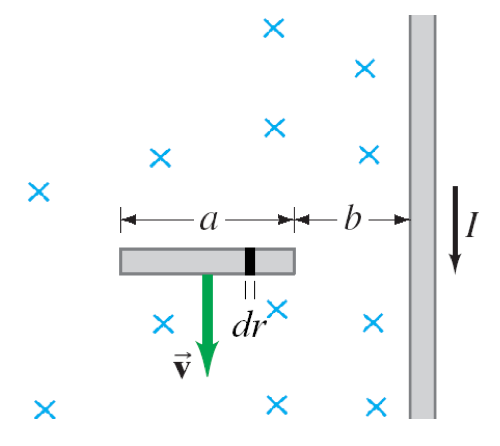
\includegraphics[scale = 0.4]{oz06/resources/Oz6Oef1-2.png}
                    \end{minipage}
            \end{description}
        \item     
            \begin{description}[labelwidth=1.5cm, leftmargin=!]
                \item[Geg. :] $v$, $I$, $a$, $b$
                \item[Gevr. :] $\mathcal{E}_{\text{ind}}$
                \item[Opl. :] Analoog aan (a), maar de emf is gericht \textbf{van} de draad.
            \end{description}
    \end{enumerate}

\vspace{1cm}